\documentclass{article}

\usepackage[english]{babel}
\usepackage[utf8]{inputenc}
\usepackage{amsmath,amssymb}
\usepackage{parskip}
\usepackage{graphicx}
\usepackage{listings}
\usepackage{float}

% Margins
\usepackage[top=2.5cm, left=3cm, right=3cm, bottom=4.0cm]{geometry}
% Colour table cells
\usepackage[table]{xcolor}

% Get larger line spacing in table
\newcommand{\tablespace}{\\[1.25mm]}
\newcommand\Tstrut{\rule{0pt}{2.6ex}}         % = `top' strut
\newcommand\tstrut{\rule{0pt}{2.0ex}}         % = `top' strut
\newcommand\Bstrut{\rule[-0.9ex]{0pt}{0pt}}   % = `bottom' strut

%%%%%%%%%%%%%%%%%
%     Title     %
%%%%%%%%%%%%%%%%%
\title{CSCI803 Project}
\author{Yao Xiao \\ SID 2019180015}
\date{\today}

\begin{document}
\maketitle

%%%%%%%%%%%%%%%%%
%   Problem 1   %
%%%%%%%%%%%%%%%%%
\section{Part 1}
\subsection{1)}
$$P'=\left\{p_1,p_2,p_3,c_1,c_2,p_4,p_5,p_6\right\}$$

$$^{\circ}P'=\left\{t_1,t_2,t_3,t_4,t_5,t_6\right\}$$

$$P'^{\circ}=\left\{t_1,t_2,t_3,t_4,t_5,t_6\right\}$$

A trap is a set of places $P′$ such that the set of output transitions of $P′$ is included in the set of input transitions of $P′$.

We have $P'^{\circ} \subseteq \ ^{\circ}P'$.

A siphon is a set of places $P′$ such that the set of input transitions of $P′$ is included in the set of output transitions of $P′$.

We have $^{\circ}P' \subseteq P'^{\circ}$.

Based on these, traps and siphons exist in the given Petri net.

\subsection{2)}
We suppose the marking of $p_2$ have passed to $p_1$, and the marking of $p_4$ have passed to $p_5$. And we use the fundamental equation to prove the features.

$$M_0 = (1,0,0,0,1,0,1,1)$$

$$s_0 = (0,1,0,0,0,0)$$

$$W = 
  \left[
  \begin{matrix}
   1 & -1 & 0 & 0 & 0 & 0\\
   -1 & 0 & 1 & 0 & 0 & 0\\
   0 & 1 & -1 & 0 & 0 & 0\\
   0 & 0 & 0 & -1 & 0 & 1\\
   0 & 0 & 0 & 1 & -1 & 0\\
   0 & 0 & 0 & 0 & 1 & -1\\
   0 & 0 & 0 & 0 & -1 & 1\\
   0 & -1 & 1 & 0 & 0 & 0
  \end{matrix}
  \right]
$$

$$M_0 + W \cdot s_0 = M$$
$$M= (0,0,1,0,1,0,1,0)$$

We can see after fundamental equation, $p_3, p_5, c_1$ have the marking, and because $c_2$ don't have the marking, so $p_6$ won't have the marking. Based on the analysis, $p_3$ and $p_6$ cannot contain one token at the same time for all reachable markings M, e mutual exclusion feature of the Petri net model is proved.



\section{Part 2}
\begin{figure}[H]
  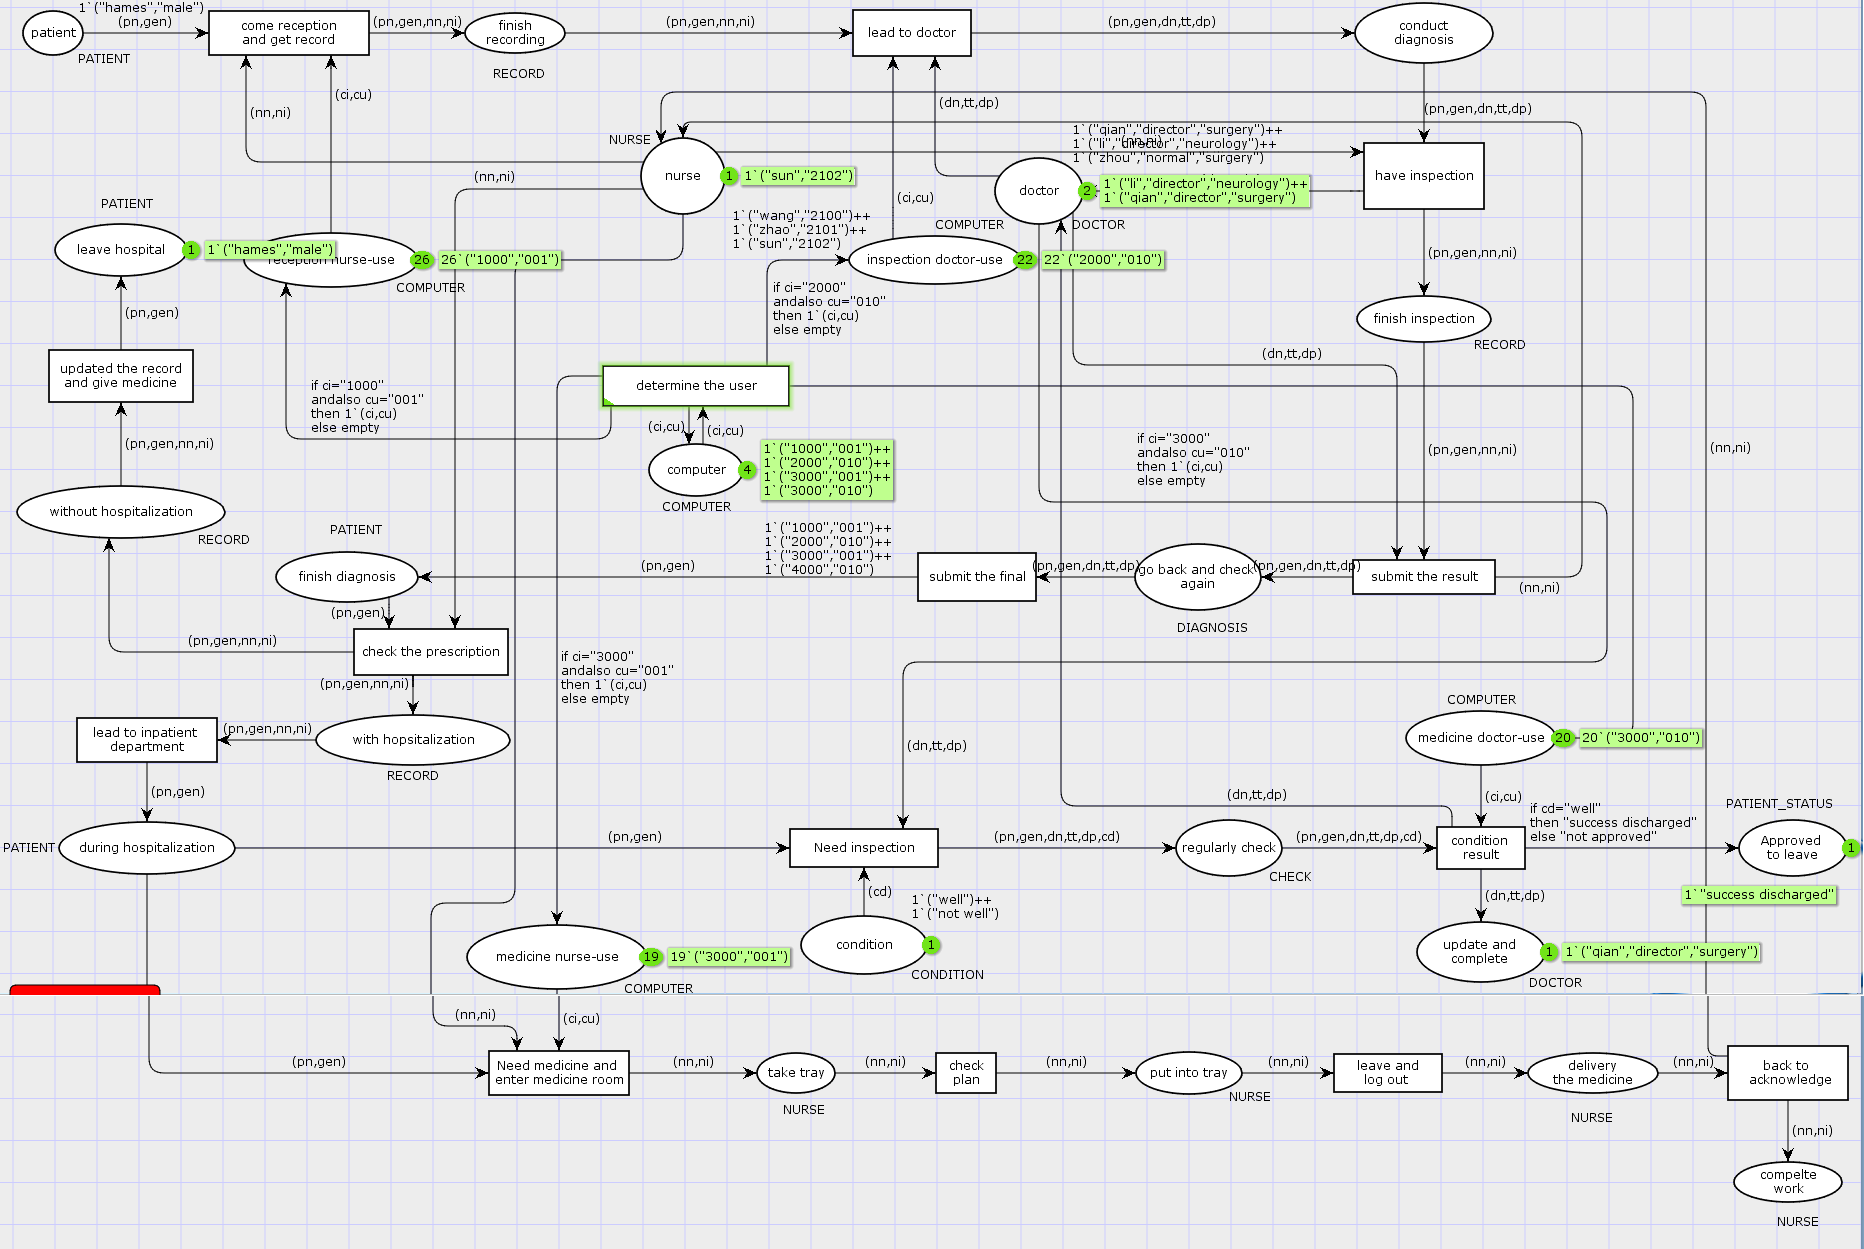
\includegraphics[width=1\textwidth]{Fig2-1}
\end{figure}

\begin{figure}[H]
  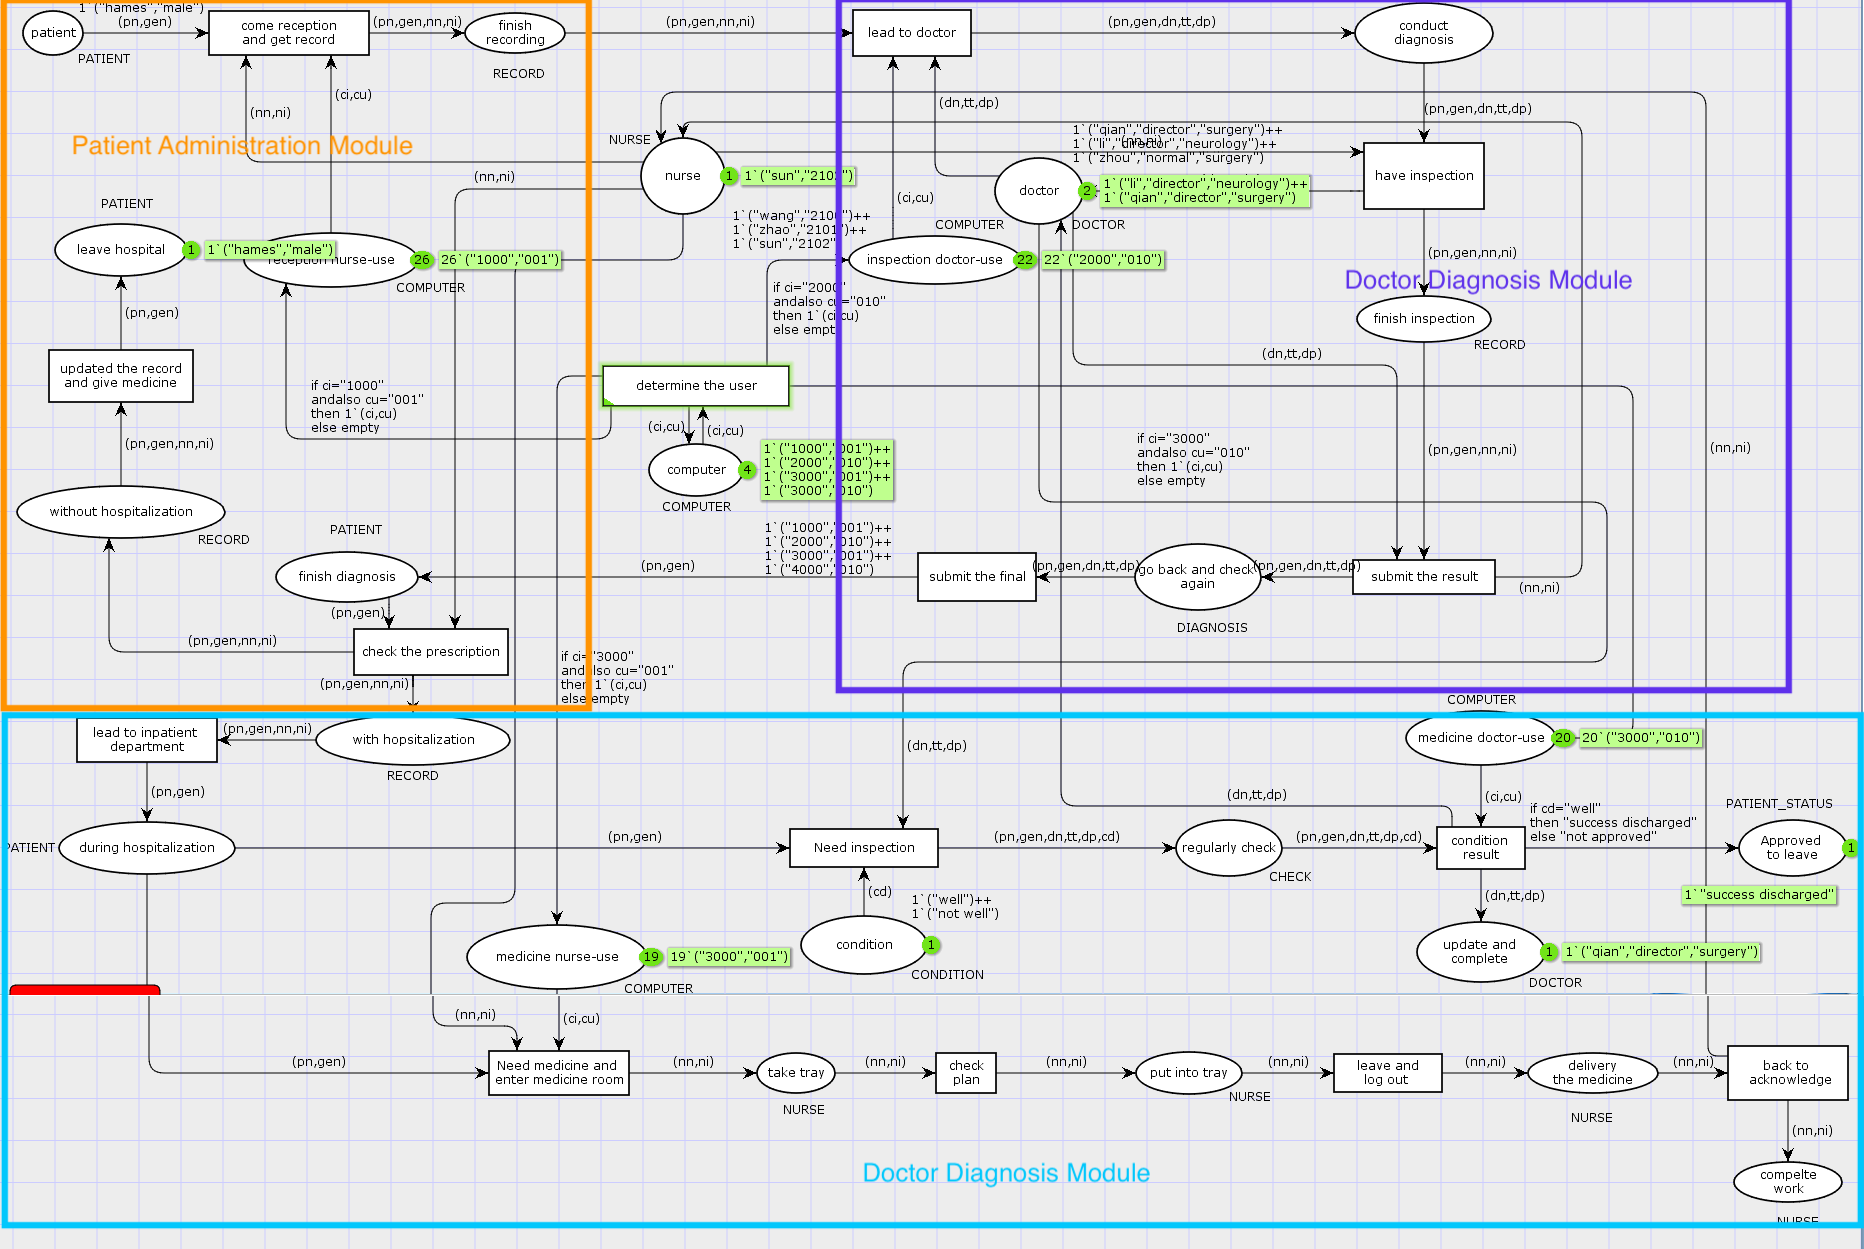
\includegraphics[width=1\textwidth]{Fig2-2}
\end{figure}

1. Set of places: P=\{patient, nurse, computer, reception nurse-use, finish recording, finish diagnosis, without hospitaliztion, doctor,
inspection doctor-use, conduct diagnosis, finish inspection, go back and check again, with hospitaliztion, during hospitaliztion, medicine nurse-use, take tray, put int tray, delivery the medicine, complete work, 
regularly check, update and complet, approved to leave, medicine doctor-use, condition\}

2. Set of transitions: T=\{come reception and get record, determine the user, check the prescription, updated the record and give medicine, lead to doctor, have inspection, submit the result, submit the final, lead to inpatient department, need inspection, condition result,
need medicine and enter medicine room, check plan, leave and log out, back to acknowledge\}

3. Set of arcs: A=\{(patient,come reception and get record), (come reception and get record,finish recording), (reception nurse-use, come reception and get record), (nurse, come reception and get record), (finish recording, lead to doctor),
(inspection doctor-use, lead to doctor), (doctor, lead to doctor), (lead to doctor, conduct diagnosis), (conduct, have inspection), $\cdots$, (back to acknowledgek, complete work)\}

4. Set of colour sets: $\sum$ = \{PATIENT, RECORD, NURSE, COMPUTER, DOCTOR, DIAGNOSIS, CONDITION, PATIENT\_STATUS\}

5. Set of variables: V=\{pn:PATIENT\_NAME, gen:GENDER, ni:NURSE\_ID, nn:NURSE\_NAME, ci:COMPUTER\_ID, 
cu:COMPUTER\_USER, dn:DOCTOR\_NAME, tt:TITLE, dp:DEPARTMENT, cd:CONDITION\}

6. Set of colour set functions: 
$$  
C(p)=\left\{
\begin{aligned}
PATIENT \quad &\mbox{if}\ p \in \left\{PATIENT\_NAME, GENDER\right\}\\
NURSE \quad &\mbox{if}\ p \in \left\{NURSE\_NAME, NURSE\_ID\right\}\\
COMPUTER \quad &\mbox{if}\ p \in \left\{COMPUTER\_ID, COMPUTER\_USER\right\} \\
DOCTOR \quad &\mbox{if}\ p \in \left\{DOCTOR\_NAME, TITLE, DEPARTMENT\right\} \\
DIAGNOSIS \quad &\mbox{if}\ p \in \left\{PATIENT\_NAME, GENDER, DOCTOR\_NAME, TITLE, DEPARTMENT\right\} \\
CONDITION \quad &\mbox{if}\ p = CONDITION\\
PATIENT\_STATUS \quad &\mbox{if}\ p = PATIENT\_STATUS\\
\end{aligned}
\right.
$$

7. Set of arc expression functions:
$$ E(a)=\left\{
\begin{array}{rcl}
1^{\prime}(pg,gen)  &      & \mbox{if}\ a \in \{(\mbox{patient, come reception and get record}),\cdots\}\\
1^{\prime}(nn,ni)  &      & \mbox{if}\ a \in \{(\mbox{nurse,come reception and get record}),\cdots\}\\
1^{\prime}(ci,cu)  &      & \mbox{if}\ a \in \{(\mbox{computer, determine the user}),\cdots\}\\
\mbox{if} \ ci=``1000"\\ \mbox{and\ also}\ cu=``001"  \\ \mbox{then}\ 1^{\prime}(ci,cu) \\ \mbox{else\ empty} &      & \mbox{if}\ a = (\mbox{determine the use, reception nurse-use}) \\
\mbox{if} \ ci=``2000"\\ \mbox{and\ also}\ cu=``010"  \\ \mbox{then}\ 1^{\prime}(ci,cu) \\ \mbox{else\ empty} &      & \mbox{if}\ a = (\mbox{determine the use, inspection doctor-use}) \\
\mbox{if} \ ci=``3000"\\ \mbox{and\ also}\ cu=``001"  \\ \mbox{then}\ 1^{\prime}(ci,cu) \\ \mbox{else\ empty} &      & \mbox{if}\ a = (\mbox{determine the use, medicine nurse-use}) \\
\mbox{if} \ ci=``3000"\\ \mbox{and\ also}\ cu=``010"  \\ \mbox{then}\ 1^{\prime}(ci,cu) \\ \mbox{else\ empty} &      & \mbox{if}\ a = (\mbox{determine the use, medicine doctor-use}) \\
1^{\prime}(dn,tt,dp)  &      & \mbox{if}\ a \in \{(\mbox{doctor, lead to doctor}),\cdots\}\\
1^{\prime}(cd)  &      & \mbox{if}\ a = (\mbox{condition, need inspection})\\
\mbox{if} \ cd=``well"\\ \mbox{then ``success discharged''} \\ \mbox{else ``not approved''} &      & \mbox{if}\ a = (\mbox{condition result, approved to leave})
\end{array} \right. $$

8. Set of initialisation functions
$$  
I(p)=\left\{
\begin{aligned}
AllPatient \quad &\mbox{if}\ p=patient\\
AllNurse \quad &\mbox{if}\ p=nurse\\
AllDoctor \quad &\mbox{if}\ p=doctor\\
AllComputer \quad &\mbox{if}\ p=computer\\
1^{\prime}(``1000'',``001'') \quad &\mbox{if}\ p=reception\ nurse-use\\
1^{\prime}(``2000'',``010'') \quad &\mbox{if}\ p=inspection\ doctor-use\\
1^{\prime}(``3000'',``001'') \quad &\mbox{if}\ p=medicine\ nurse-use\\
1^{\prime}(``3000'',``010'') \quad &\mbox{if}\ p=medicine\ doctor-use\\
1^{\prime}``\; " \quad &\mbox{if}\ p=approved to leave\\
1^{\prime}(``well")\ \mbox{and}\ 1^{\prime}(``not well") \quad &\mbox{if}\ p=condition\\
\end{aligned}
\right.$$

\section{Part 3}
\begin{figure}[H]
  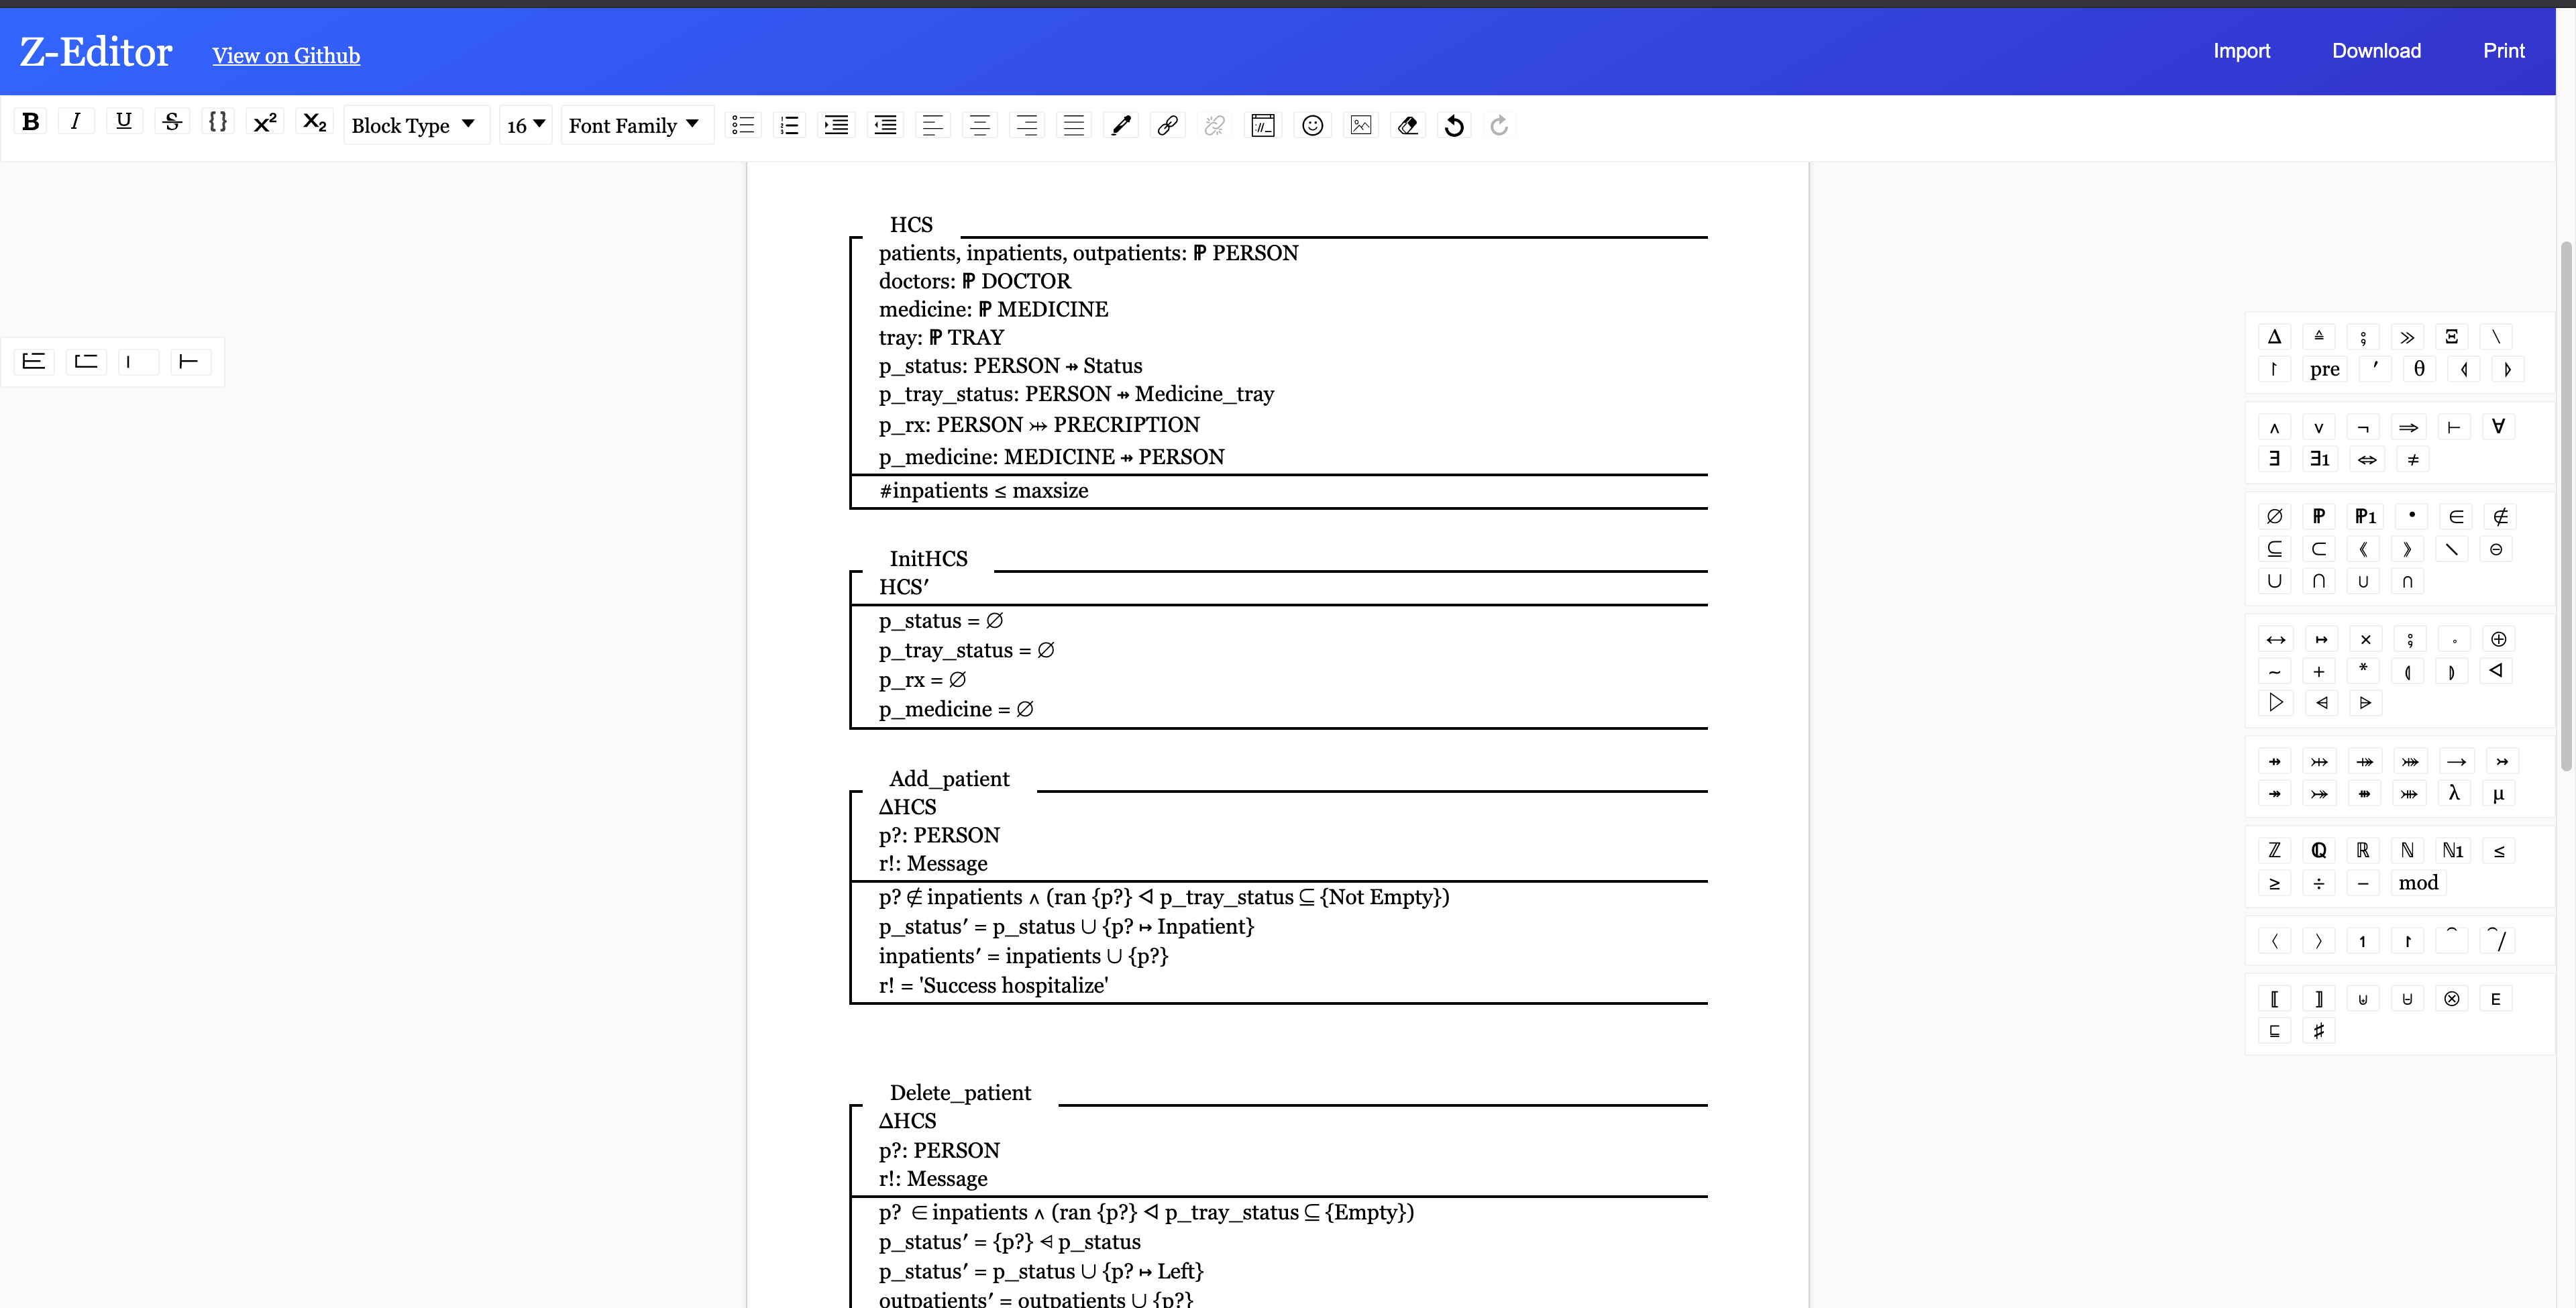
\includegraphics[width=1\textwidth]{Fig3}
\end{figure}

\end{document}


